\section{Methodology}\label{sec:chp6:method}

Our \ac{mpmri} \ac{cad} system consists of seven different steps: pre-processing, segmentation, registration, feature detection, balancing, feature selection/extraction, and finally classification.
%% It should be noted that \ac{cad} system designed deals with multiparametric \ac{mri} data. 

\subsection{Pre-processing}\label{subsec:chp6:method:PP}

\begin{figure}
  \hspace*{\fill}
  \subfigure[]{\label{fig:adcpdf1}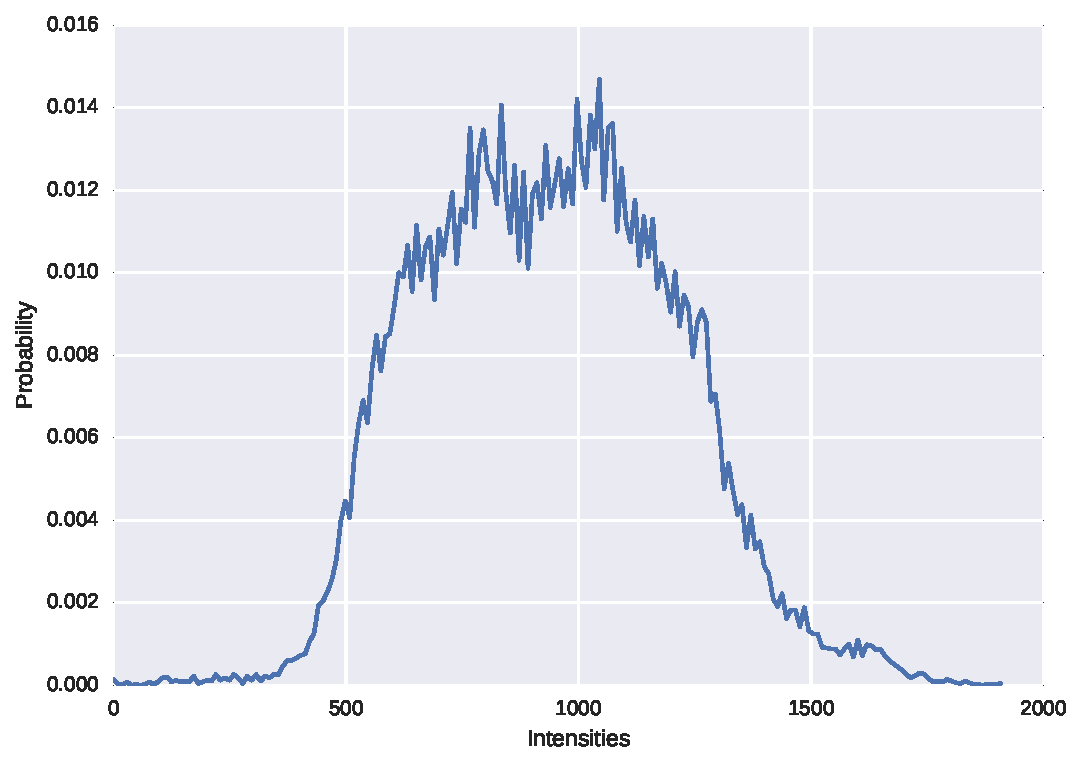
\includegraphics[width=.3\textwidth]{6_pipeline/figures/adc_pdf.pdf}}
  \hfill
  \subfigure[]{\label{fig:adcpdf2}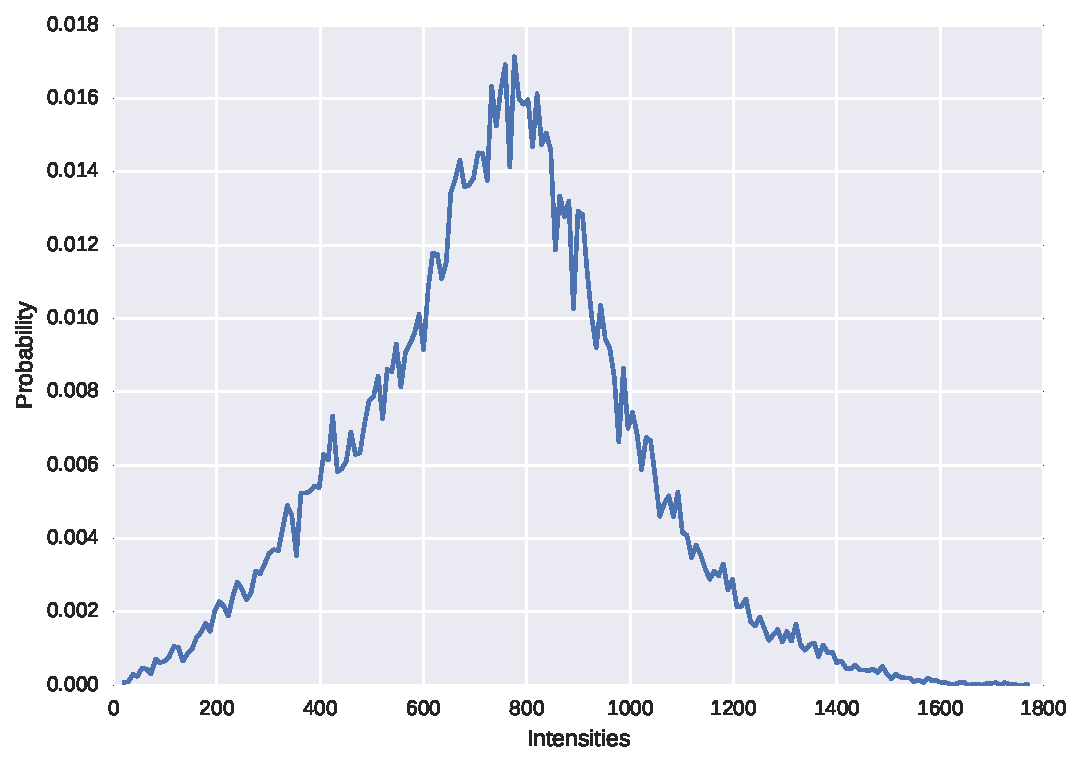
\includegraphics[width=.3\textwidth]{6_pipeline/figures/adc_pdf_2.pdf}}
  \hfill
  \subfigure[]{\label{fig:adcpdf3}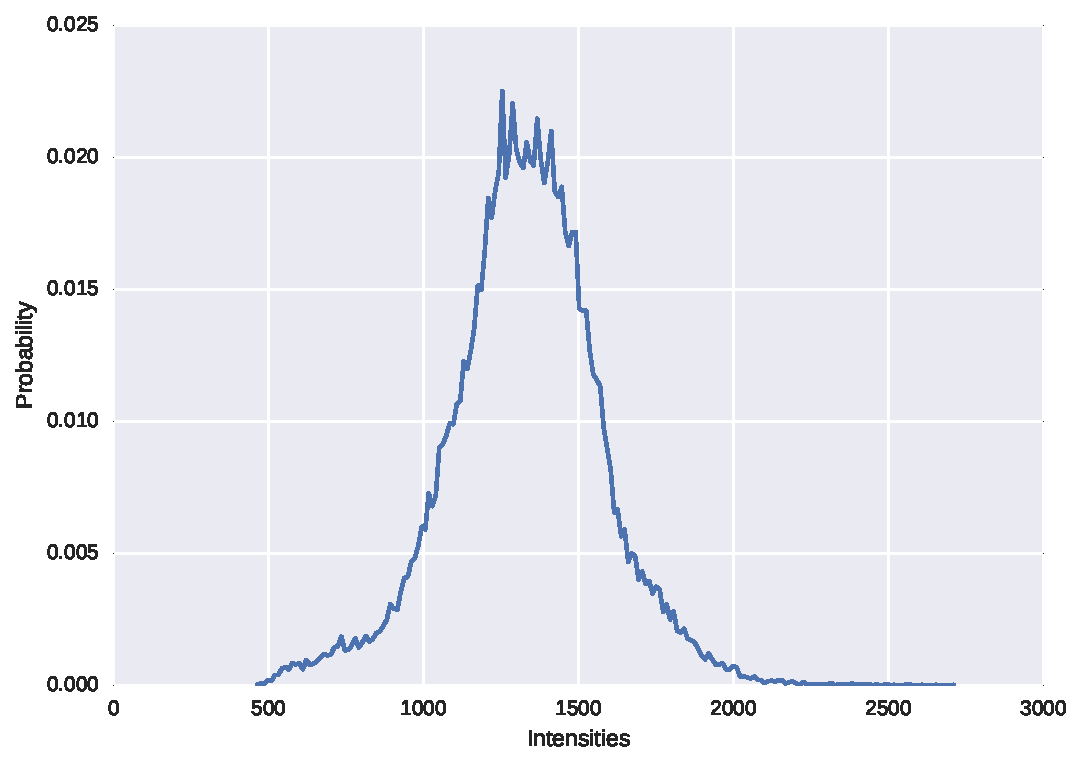
\includegraphics[width=.3\textwidth]{6_pipeline/figures/adc_pdf_3.pdf}}
  \hspace*{\fill}
  \caption[Illustration of the \acs*{pdf} of the \acs*{adc} coefficients within the prostate.]{Illustration of the variability of the \acs*{pdf} of the \acs*{adc} coefficients within the prostate for 3 patients.}
  \label{fig:adcpdf}
\end{figure}


The reader can refer to \acs{sec}\,\ref{subsec:chp3img-reg:prepro} to have an extensive overview of the state-of-the-art methods used to pre-process \ac{mpmri} data.
Three types of pre-processing are used for \ac{mri} images: (i) noise filtering, (ii) bias correction, and (iii) standardization/normalization.
Our dataset is based on \SI{3}{\tesla} images without endorectal coil and therefore, the two first types of correction have not been considered as necessary.
Normalization is, however, a crucial step to reduce the inter-patient variations which allows to improve the learning during the classification stage.
\Ac{chp}~\ref{chap:5} presented two normalization methods to pre-process \ac{t2w}-\ac{mri} and \ac{dce}-\ac{mri}, respectively.
Therefore, we used these methods to standardize these images.
Regarding the \ac{adc} map normalization, the \ac{pdf} within the prostate does not follow a known distribution as depicted in \acs{fig}\,\ref{fig:adcpdf}.
Thus, one cannot use a parametric model to normalize these images and a non-parametric piecewise-linear normalization~\cite{Nyul2000} is the best option for this case.

Additionally, the \ac{mrsi} modality requires a specific pre-processing based on signal processing rather than image processing.
Therefore, the \ac{mrsi} modality has been pre-processed to correct the phase, baseline, and frequency.
Regarding the problem of phase correction and frequency alignment, we use the most efficient method of the state-of-the-art review in \acs{sec}\,\ref{subsec:chp3img-reg:prepro}.
Indeed, as \citeauthor{Parfait2012} and \citeauthor{trigui2017automatic}~\cite{Parfait2012,trigui2016classification,trigui2017automatic}, the phase of each \ac{mrsi} spectra is corrected using the approach of \citeauthor{Chen2002}~\cite{Chen2002}.
Along the same line, the frequency shift of each spectra is corrected by aligning to \SI{4.65}{\ppm} the maximum of an inferred function fitted to the residuals of water, using a Voigt profile as in \acs{eq}\,\eqref{eq:voigt}.

\begin{equation}
  V(x; \sigma, \gamma) = \frac{\mathbf{R} \left[ w(z) \right]}{\sigma \sqrt{2\pi}} \ ,
  \label{eq:voigt}
\end{equation}

\noindent where $\mathbf{R} \left[ w(z) \right]$ is the real part of the Faddeva function for $z = \frac{x + i \gamma}{\sigma \sqrt{2}}$.

By assessing the qualitative results obtained in~\cite{Parfait2010}, the baseline correction method used by \citeauthor{Parfait2012} and \citeauthor{trigui2017automatic} does not provide an optimal solution for that matter.
The iterative low-pass filter enforces too much the smoothness of the baseline.
\citeauthor{xi2008baseline} proposed a baseline detection derived from a parametric smoothing model~\cite{xi2008baseline}.
The \ac{nmr} signal is formalized as a sum of a pure signal, the baseline function, and an additive Gaussian noise such as:

\begin{equation}
  y_i = b_i + \mu_i e^{n_i} + \varepsilon_i \ ,
  \label{eq:methodBaselineDetectionModel}
\end{equation}

\noindent where $y_i$ is the \ac{nmr} signal, $b_i$ is the baseline, $\mu_i$ is the true signal, and $n_i$ and $\varepsilon_i$ are Gaussian noises.

\citeauthor{xi2008baseline} propose to find the baseline function through an iterative optimization by maximizing the following cost function:

\begin{equation}
  F(b) = \sum_{i = 1}^{N} b_i - \frac{A^{*} N^4}{\sigma} \sum_{i = 1}^{N} (b_{i+1} + b_{i-1} - 2 b_i)^2 - \frac{1.25 B^{*}}{\sigma} \sum_{i = 1}^{N} (b_i - \gamma_i)^2 g(b_i - \gamma_i) \ ,
  \label{eq:methodBaselineDetectionCostFunction}
\end{equation}

\noindent where $g(b_i - \gamma_i)$ is the Heaviside function, $A^*$ and $B^*$ are the terms controlling the smoothness and negative penalties, respectively, $\sigma$ is an estimation of the standard deviation of the noise, and $N$ is the total number of points in the \ac{mrsi} signal.

The standard deviation of the noise $\sigma$ is estimated as in~\cite{xi2008baseline}, and the $A^{*}$ and $B^{*}$ are empirically set to $5 \times 10^{-6}$ and $100$, respectively, for all the \ac{mrsi} signal.
Setting these parameters allows to obtain an estimation of a smooth and possibly negative baseline, required by the aspect of the citrate peak in our \ac{mrsi} acquisition, as depicted in \acs{fig}\,\ref{fig:baselinemrsi}.

\begin{figure}
  \centering
  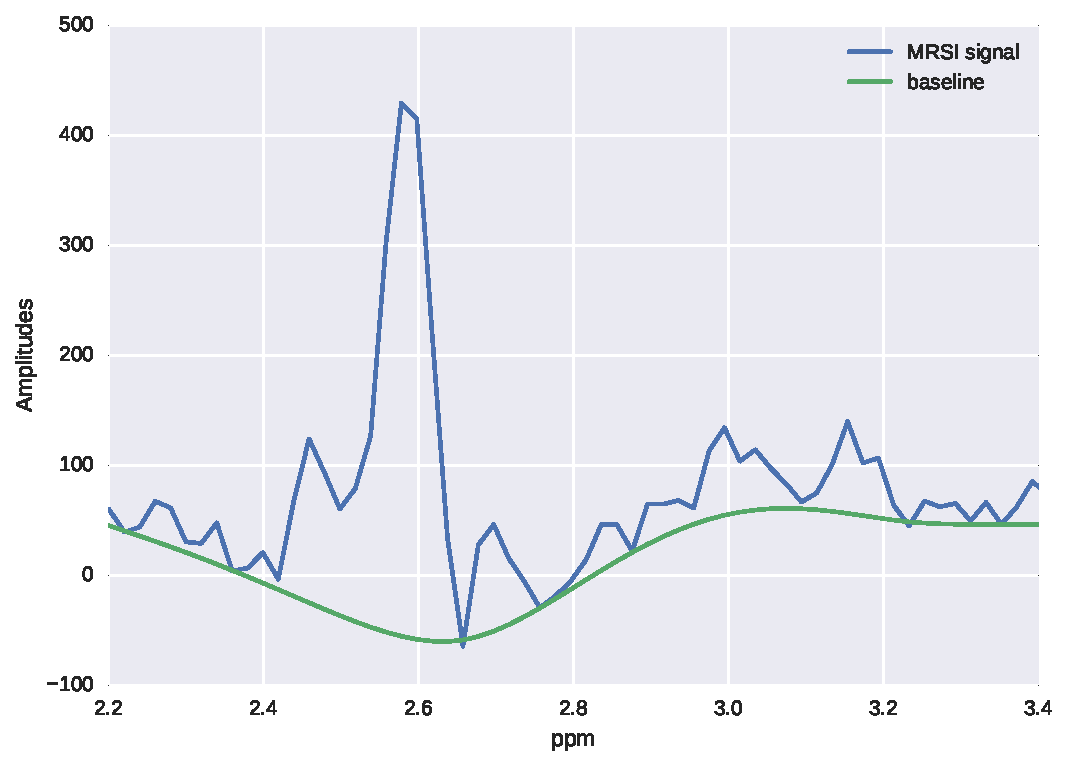
\includegraphics[width=0.5\linewidth]{6_pipeline/figures/baseline_mrsi.pdf}
  \caption{Illustration of the detection of the baseline on an \acs*{mrsi} spectrum.}
  \label{fig:baselinemrsi}
\end{figure}

Additionally, each \ac{mrsi} spectrum is normalized using the L$_2$ norm, which has been shown to be the most efficient normalization method in \ac{mrsi} as discussed in \acs{sec}\,\ref{subsec:chp3img-reg:prepro}.

\subsection{Segmentation and registration}\label{subsec:chp6:method:Seg-Reg}

For this study, no segmentation method has been developed and the manual segmentation given by our radiologist has been used.
The prostate is suffering, however, from a misalignment between the different \ac{mri} modalities.
Therefore, three registrations have been developed to: (i) the patient motion during the \ac{dce}-\ac{mri} acquisition, (ii) the patient motion between the \ac{t2w}-\ac{mri} and the \ac{dce}-\ac{mri} acquisitions, and (iii) the patient motion between the \ac{t2w}-\ac{mri} and the \ac{adc} map acquisition.
All registrations are implemented in C++ using \ac{itk}.

The \ac{dce}-\ac{mri} acquisition being dynamic, some intra-patient might occur during the acquisition.
For each serie of this dynamic acquisition, each 3D volume is registered to the first volume acquired, to remove the residual motion.
The appearance in the \ac{dce}-\ac{mri} images, however, varies due to the presence or not of the contrast media.
Therefore, the metric chosen to be minimized is the \ac{mi} and the geometric transform has been set to a rigid transform.
The optimization is performed using a regular step gradient descent.

Once the intra-patient motions corrected, a registration to correct the alignment between the \ac{t2w}-\ac{mri} and the \ac{dce}-\ac{mri} acquisitions is performed.
For that matter, the prostate has been segmented in both modalities --- \ac{t2w}-\ac{mri} and \ac{dce}-\ac{mri} --- to create two binary masks.
Therefore, these 3D binary masks are directly registered using the \ac{mse} metric.
Unlike the previous registration, we use a more complex geometric transform by successively finding a rigid transformation, a coarse elastic transformation, and a fine elastic transformation.
B-splines transformation is used as the elastic transform.
These successive transformations allow to get a good initialization for the next transformation.
The transformation is inferred by minimizing the cost function using a regular step gradient descent.

The \ac{t2w}-\ac{mri} and \ac{adc} map acquisitions are identically registered than the the \ac{t2w}-\ac{mri} and the \ac{dce}-\ac{mri} modalities.
Additionally, the \ac{cap}, \ac{pz}, and \ac{cg} are segmented on the \ac{t2w}-\ac{mri} and thus the latter modality is used as the reference modality.

\subsection{Feature detection}\label{subsec:chp6:method:fea-det}

\begin{table}
  \caption{Features extracted in \acs*{t2w}-\acs*{mri} and \acs*{adc} volumes.}
  \centering
  \scriptsize
  \begin{tabularx}{\textwidth}{lXc}
    \toprule
    \textbf{Features} & \textbf{Parameters} & \textbf{\# dimensions} \\
    \midrule
    Intensity &  & 1 \\
    \acs*{dct} decomposition & window: \SI[product-units=repeat]{9x9x3}{\px} & 243 \\
    Kirsch filter &  & 2 \\
    Laplacian filter &  & 1 \\
    Prewitt filter &  & 3 \\
    Scharr filter &  & 3 \\
    Sobel filter &  & 3 \\
    Gabor filters & 4 frequencies $f \in [0.05, 0.25]$; 4 azimuth angles $\alpha \in [0, \pi]$; 8 elevation angles $\alpha \in [0, 2\pi]$ & 256 \\
    Phase congruency filter & 5 orientations; 6 scales & 3 \\
    Haralick filter & window: \SI[product-units=repeat]{9x9x3}{\px}; \# grey levels: 8; distance: \SI{1}{\px}; 13 directions & 169 \\
    \acs*{lbp} filter & 2 radii $r=\{1, 2\}$; 2 neighborhood sizes $N = \{8, 16\}$ & 6 \\
    \bottomrule
  \end{tabularx}
  \label{tab:featureadct2w}
\end{table}

To approach the task of automatic detection of \ac{cap} using machine learning, one has to extract a variety of feature specific to the \ac{mri} modality as presented in \acs*{sec}\,\ref{subsec:chp3:img-clas:CADX-fea-dec}.

\paragraph{\ac{t2w}-\ac{mri} and \ac{adc} map features}
Apart of using the normalized intensity, edge- and texture-based features are commonly extracted from \ac{t2w}-\ac{mri} and \ac{adc} map.
A set of common features earlier reported in \acs*{sec}\,\ref{subsec:chp3:img-clas:CADX-fea-dec} have been computed.
The following set of filters characterizing edges have been used: (i) Kirsch, (ii) Laplacian, (iii) Prewitt, (iv) Scharr, (v) Sobel, and (vi) Gabor.
Apart of Kirsch filter, the other filters are applied in 3D to get more information using a volume and not a slice, as it is usually done.
The extension of the most common edge detectors in 3D is obvious and will not be recalled.
However, 3D Gabor filters~\cite{wang2005face} are not commonly used and we recall their formulation in \acs*{eq}\,\eqref{eq:gabor3d}.

\begin{equation}
  g(\mathbf{x};\boldsymbol{\sigma},f,\theta,\phi) = \hat{g}(\mathbf{x};\boldsymbol{\sigma}) \exp(j 2 \pi f \left( x \sin \theta \cos \phi + y \sin \theta \sin \phi + z \cos \theta \right)) \ ,
  \label{eq:gabor3d}
\end{equation}

\noindent where,

\begin{equation}
  \hat{g}(\mathbf{x};\boldsymbol{\sigma}) = \frac{1}{{\left(2 \pi\right)}^{\frac{3}{2}}} \exp \left( -\frac{1}{2} \left( \frac{x^2}{\sigma_x^2} + \frac{y^2}{\sigma_y^2} + \frac{z^2}{\sigma_z^2} \right) \right) \ ,
  \label{eq:gabor3dgaussian}
\end{equation}

\noindent where $\mathbf{x}$ is the position vector $\{x,y,z\}$, $\boldsymbol{\sigma}$ is the standard deviation vector $\{\sigma_x,\sigma_y,\sigma_z\}$ of the 3D Gaussian envelope, $f$ is the radial center frequency of the sine wave, $\theta$ is the elevation angle, and $\phi$ is the azimuth angle.

Additionally, features based on phase congruency as proposed by \citeauthor{kovesi1999image} are computed~\cite{kovesi1999image}.
Therefore, from a set of Log-Gabor filter bank, the orientation image, the local weighted mean phase angle, and the phase angle are estimated at each voxel.

To characterize the local texture, both second-order \ac{glcm}-based features~\cite{Haralick1973} and rotation invariant and uniform \ac{lbp}~\cite{ojala2002multiresolution} are extracted.
To encode 3D information, the 13 first Haralick features --- refer to \acs{tab}~\ref{tab:glcm} --- are computed for the 13 possible directions.
For the same reason, the \ac{lbp} codes are computed for the three-orthogonal-planes of each \ac{mri} volume.

\Acl{tab}~\ref{tab:featureadct2w} summarizes the different features extracted with their corresponding parameters.
Note that all these features are extracted at each voxel of the volume.

\paragraph{\ac{dce}-\ac{mri} features} The extracted features for the \ac{dce}-\ac{mri} are exactly the same than in the previous chapter.
The reader can refer to \ac{sec}\,\ref{subsubsec:chp5:DCE-norm:stateart} for a detailed presentation of the different methods used.
In brief, the entire enhanced signal, semi-quantitative, and quantitative methods are computed. 

\begin{figure}
  \hspace*{\fill}
  \subfigure[]{\label{fig:goodfit}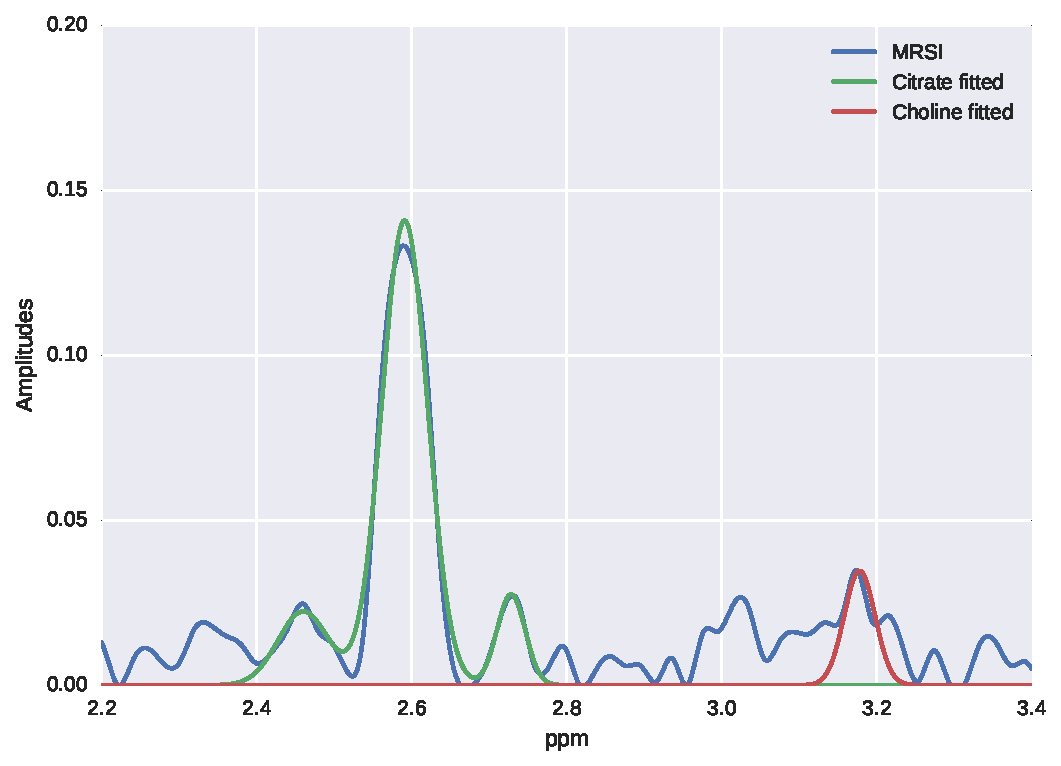
\includegraphics[width=.49\textwidth]{6_pipeline/figures/meta_fitting.pdf}}
  \hfill
  \subfigure[]{\label{fig:wrongfit}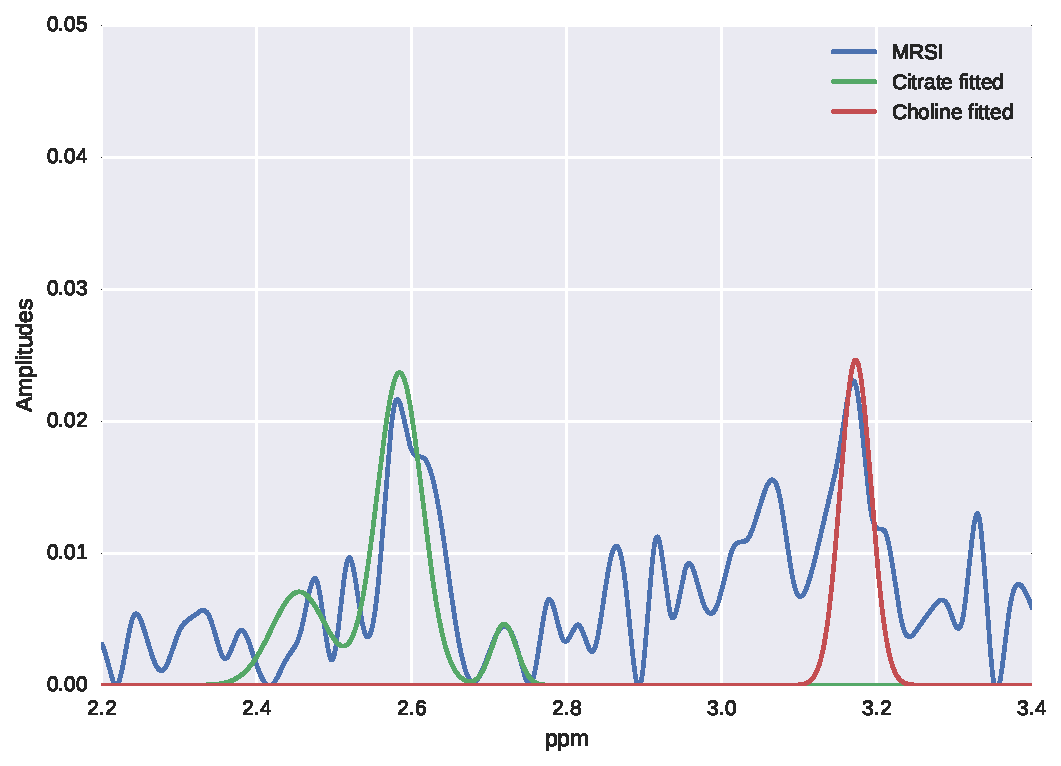
\includegraphics[width=.49\textwidth]{6_pipeline/figures/meta_fitting_wrong.pdf}}
  \hspace*{\fill}
  \caption[Illustration of the metabolite fitting.]{Illustration of the metabolite fitting: \subref{fig:goodfit} the models are perfectly fitted for both citrate and choline; \subref{fig:wrongfit} the fitting of the citrate metabolite is inaccurate since it does not follow the \textit{a priori} model.}
  \label{fig:fitmeta}
\end{figure}

\paragraph{\ac{mrsi} features} \ac{mrsi}-based features have been explained in \acs{sec}\,\ref{subsubsec:chp3:img-clas:CADX-fea-dec:MRSI-fea}.
Due to unavailability of some unsuppressed water acquisition, absolute quantification as presented by \citeauthor{trigui2017automatic} could not be computed~\cite{trigui2017automatic}.
Therefore, likewise in~\cite{Parfait2012}, three different techniques are used to extract discriminative features: (i) relative quantification based on metabolite quantification, (ii) relative quantification based on bounds integration, and (iii) spectra extraction.

Relative quantification based on metabolite quantification relies on a robust integration of the citrate and choline signal based on peak modelling.
Therefore, we propose to tackle this problem as a non-linear least squares optimization problem by (i) quantifying the citrate peaks as a Gaussian mixture and (ii) quantifying the choline as a single Gaussian.

As illustrated in \acs{fig}\,\ref{fig:goodfit}, the \ac{mrsi} sequence imply a 3-peaks citrate metabolite.
Therefore, we propose the following cost function to represent our function as in \acs{eq}\,\eqref{eq:costcit}.

\begin{equation}
  C_1(x; \mathbf{w}) = \alpha_1 \mathcal{N}(x; \mu, \sigma_1) + \alpha_2 \mathcal{N}(x; \mu + \delta_2, \sigma_2) + \alpha_3 \mathcal{N(x; \mu - \delta_3, \sigma_3)} \ ,
  \label{eq:costcit}
\end{equation}

\noindent where $\mathcal{N}(\cdot)$ is a Gaussian distribution, $\mu$ is the central mean of the citrate, $\delta_2$ and $\delta_3$ are the shifts from the citrate central peak to the citrate side peaks, $\{\alpha_1, \alpha_2, \alpha_3\}$ are the amplitude factors of each Gaussian distribution, and $\{\sigma_1, \sigma_2, \sigma_3\}$ are the standard deviations of each Gaussian distribution. Additionally, we defined $\mathbf{w}$ as the vector containing the free parameters.

\Acl{eq}~\eqref{eq:costcit} is minimized under constraints as in \acs{eq}\,\eqref{eq:mincostcit}.


\begin{equation}
\begin{aligned}
& \argmin_{\mathbf{w}} 
& & | S(x) - C_1(x; \mathbf{w}) |^{2} \ , \label{eq:mincostcit} \\
& \text{subject to}
& & 2.54 < \mu < 2.68 \ , \\
&&& 0.06 < \delta_1, \delta_2 < 0.16 \ , \\
&&& 0.01 < \sigma_1, \sigma_2, \sigma_3 < 0.1 \ , \\
&&& \alpha_1, \alpha_2, \alpha_3 > 0 \ ,
\end{aligned}
\end{equation}

\noindent where $S(x)$ is the \ac{mrsi} signal. The different constraints are empirically set but based on the \emph{a priori} location of the peaks.

\Acl{fig}~\ref{fig:fitmeta} illustrates two fitting cases.
If the \ac{mrsi} signal follows the assumption regarding the model, which is generally the case --- i.e., a mixture of 3 Gaussian distributions ---, the signal is perfectly fitted as shown in \acs{fig}\,\ref{fig:goodfit}.
However, if the \ac{mrsi} signal does not obey to the model, the signal is fitted inaccurately as depicted in \acs{fig}\,\ref{fig:wrongfit}.

Theoretically, one could suggest to fit a Voigt mixtures instead of a Gaussian mixtures due to the presence of noise during the acquisition.
However, the use of Gaussian distributions reduces the number of parameters to be optimized and allows for a more robust optimization due to less interdependence between the bounds.

The choline metabolite is quantified on a similar manner assuming that there is only a single Gaussian distribution rather than a mixture.
Therefore the problem is formulated as:

\begin{equation}
  C_2(x; \mu, \sigma) = \alpha \mathcal{N}(x; \mu, \sigma) \ ,
  \label{eq:costcho}
\end{equation}

\noindent where $\mathcal{N}(\cdot)$ is a Gaussian distribution, $\mu$ is the center of the choline, $alpha$ is the amplitude factor, and $\sigma$ is the standard deviation. The optimization is performed such as:

\begin{equation}
\begin{aligned}
& \argmin_{\mathbf{\mu, \sigma}} 
& & | S(x) - C_2(x; \mu, \sigma) |^{2} \ , \label{eq:mincostcho} \\
& \text{subject to}
& & 3.17 < \mu < 3.21 \ , \\
&&& 0.001 < \sigma < 0.02 \ , \\
&&& \alpha > 0 \ .
\end{aligned}
\end{equation}

Finally, the citrate and choline fitted function are integrated to obtain the relative concentration of each metabolite.
Additionally, the ratio of the citrate over the choline is also computed.

A second solution to compute the relative concentration of each metabolite is proposed for the sake of comparison.
For both the choline and citrate, a local maximum is found near of the theoretical position of the peak.
Subsequently, a range is defined around each peak ---i.e., \SI{0.36}{\ppm} for the citrate and \SI{0.08}{\ppm} for the choline --- and the integral of the signal is computed using the Simpson's rule.

The third and last option correspond on a cropping of the \ac{mrsi} signal from \SIrange{2}{4}{\ppm}.

\paragraph{Anatomical features}

Beside the aforementioned features specific at each modality, anatomical features as proposed by \citeauthor{Chen2002} and \citeauthor{Litjens2014} are computed~\cite{Chen2002,Litjens2014}.
Therefore, 4 different metrics are computed based on the relative distance to the prostate boundary as well as the prostate center, and the relative position in the Euclidean and cylindrical coordinate systems.

\subsection{Feature balancing}\label{subsec:chp6:method:fea-bal}
Data imbalanced is a recurrent issue in classification, notably in medical data.
The problem of imbalanced dataset lies in the fact that one of the class has a smallest number of data --- i.e., in medical data, the class corresponding to patients with a disease --- compared with the other classes.
Therefore, solving the problem of imbalanced is equivalent to under- or over-sampling part of the dataset to obtain equal number of samples in the different classes.
In this section, several methods which will be used in the experiments are presented.

\subsubsection{\Acl*{us1}}
Techniques that reduce the number of samples of the majority class to be equal to the number of samples of minority class are referred as \ac{us1} techniques.
%Considering the problem of imbalanced, \ac{us} is performed such that the number of samples of the majority class is reduced to be equal to the number of samples of the minority class.

\begin{description}
  \item[\Ac{nm}] offers three different methods to under-sample the majority class~\cite{mani2003knn}.
In \ac{nm1}, samples from the majority class are selected such that for each sample, the average distance to the $k$ \ac{nn} samples from the minority class is minimum.
\ac{nm2} diverges from \ac{nm1} by considering the $k$ farthest neighbours samples from the minority class.
In \ac{nm3}, a subset $M$ containing samples from the majority class is generated by finding the $m$ \ac{nn} from each sample of the minority class.
Then, samples from the subset $M$ are selected such that for each sample, the average distance to the $k$ \ac{nn} samples from the minority class is maximum.
In our experiment, $k$ and $m$ are fixed to 3.
\item[\Ac{iht}] select samples with a high hardness threshold~\cite{smith2014instance}.
Hardness indicates the likelihood of mis-classification rate for each samples.
The notation of instance hardness are drawn through the decomposition of $p(h \vert t)$ using Bayes' theorem, where $h$ represent the mapping function used to map input features to their corresponding labels and $t$ represents the training set.
\begin{equation}
  IH_h(\langle x_{i}, y_{i}\rangle) = 1 - p(y_i \vert x_i, h).\
\label{eq:iht}
\end{equation}
Therefore, under-sampling is performed by keeping the most probable samples --- i.e, filtering the samples with high hardness value --- through \ac{kcv} training sets while considering specific threshold for filtering.
%% The hardness of an instance is depedent on the instances in the training data and the algorithm used to produced h (h is a function mapping input features to their corresponding label , i.e, the classifier, or base learner function).

 
\end{description}

\subsubsection{\Acl*{os}}
In the contrary to \ac{us1} techniques, data can be balanced by \ac{os} in which the new samples belonging to the minority class are generated, aiming at equalizing the number of samples in both classes.

\begin{description}
\item[\Ac{smote}] is a method to generate synthetic samples in the feature space~\cite{chawla2002smote}.
Let define $x_i$ as a sample belonging to the minority class.
Let define $x_{nn}$ as a randomly selected sample from the $k$-\ac{nn} of $x_i$, with $k$ set to 3.
A new sample $x_j$ is generated such that $x_j = x_i + \sigma \left( x_{nn} - x_i \right)$, where $\sigma$ is a random number in the interval $\left[0,1\right]$.
\item[\Ac{smoteb1}] over-samples the minority class similarly to \ac{smote}~\cite{han2005borderline}.
However, instead of using all the minority samples, it focuses on the borderline samples of minority class.
Borderline samples simply indicate the samples that are closer to the other class.
First, the borderline samples of minority class are detected.
A sample $x_{i}$ belongs to borderline samples if more than half of its $k$-\ac{nn} samples belong to the majority class.
Synthetic data is then created based on \ac{smote} method for borderline samples, by selecting 
Then, $s$-\ac{nn} of the minority class are selected to generate synthetic sample similarly to \ac{smote}.
 
\item[\Ac{smoteb2}] performs similarly to \ac{smoteb1}~\cite{han2005borderline}.
However, the $s$-\ac{nn} are not computing by only considering the minority class but by considering both classes.
The same generation rules as \ac{smote} is used.
\end{description}

\subsection{Feature selection and extraction}\label{subsec:chp6:method:fea-sel}


Feature selection and extraction are used in the experiment: (i) signal-based data --- i.e., \ac{mrsi} and \ac{dce}-\ac{mri} --- are decomposed using feature extraction methods while (ii) image-based features are selected through different feature selection methods.
These methods have been presented in \acs{sec}\,\ref{subsec:chp3:img-clas:CADX-fea-ext}.

Among those, \ac{pca}, sparse-\ac{pca}, and \ac{ica} are used to decompose signal-based data.

Similarly to \ac{pca} decomposition, \ac{ica} is projecting data on independent components~\cite{comon1994independent}.
However, it does not require orthogonality of the space and does not assume Gaussian distribution for each independent source.
Therefore, opposite to \ac{pca} it can recover uniquely the signals themselves rather than linear subspace in which the signals lie~\cite{murphy2012machine}.

Sparse-\ac{pca} is another approach for feature extraction and dimension reduction~\cite{zou2006sparse}.
Similarly to \ac{pca}, this approach project the data as a linear combination of input data.
However, instead of using original data, it uses a sparse representation of the data, and therefore projects them as linear combination of few input components rather than all of them.
Referring to \acs{eq}\,\eqref{eq:eigpca}, the cost function of sparse-\ac{pca} is formulated to maximize the variance while maintaining the sparsity constraint:

\begin{eqnarray}
 && \argmax \quad   \mathbf{v}^{-1} \Sigma \mathbf{v}\ , \label{eq:sparsepca}\\ 
 && \text{subject to }  \Vert \mathbf{v} \Vert_{2} = 1\ , \nonumber \\
 && \Vert \mathbf{v} \Vert_{0} \leq k\ . \nonumber
\end{eqnarray}
\noindent where $k$ indicates that number of non-zero elements in $\mathbf{v}$.

Additionally to feature extraction, we use two methods of feature selection during the experiments.
The first feature selection is the one-way \ac{anova} test.
This test is based on computing the F-test which is the ratio of the between-group variability over the with-in group variability.
The F-value is computed for each pair of feature and the $K$ feature dimensions corresponding to the largest F-values are kept.

Apart of using \ac{rf} as our main classifier, \ac{rf} provide information regarding the importance of each feature.
The feature importance in \ac{rf} is linked with the Gini importance.
In a tree classifier, the Gini impurity criterion of the child nodes is inferior to the parent node.
For each individual feature, adding the decrease of the Gini impurity along the tree gives information about the feature importance: the higher, the better.
Therefore, one can add the decrease of the Gini impurity across all the trees of a forest and obtain the importance of a specific feature for this forest.
Subsequently, the $K$ most important features are selected to perform the feature selection.

\subsection{Classification}\label{subsec:chp6:method:clas}
Variety of classifiers have been explained in \acs{sec}\,\ref{subsec:chp3:img-clas:CADX-clas}. 

Among those, \ac{rf} showed its reliability to lead to high classification performance.
That is why, \ac{rf} has been chosen to as our base classifier --- allowing for feature selection as well --- to perform classification of individual modality as well as the combination of modalities.

\begin{figure}
  \centering
  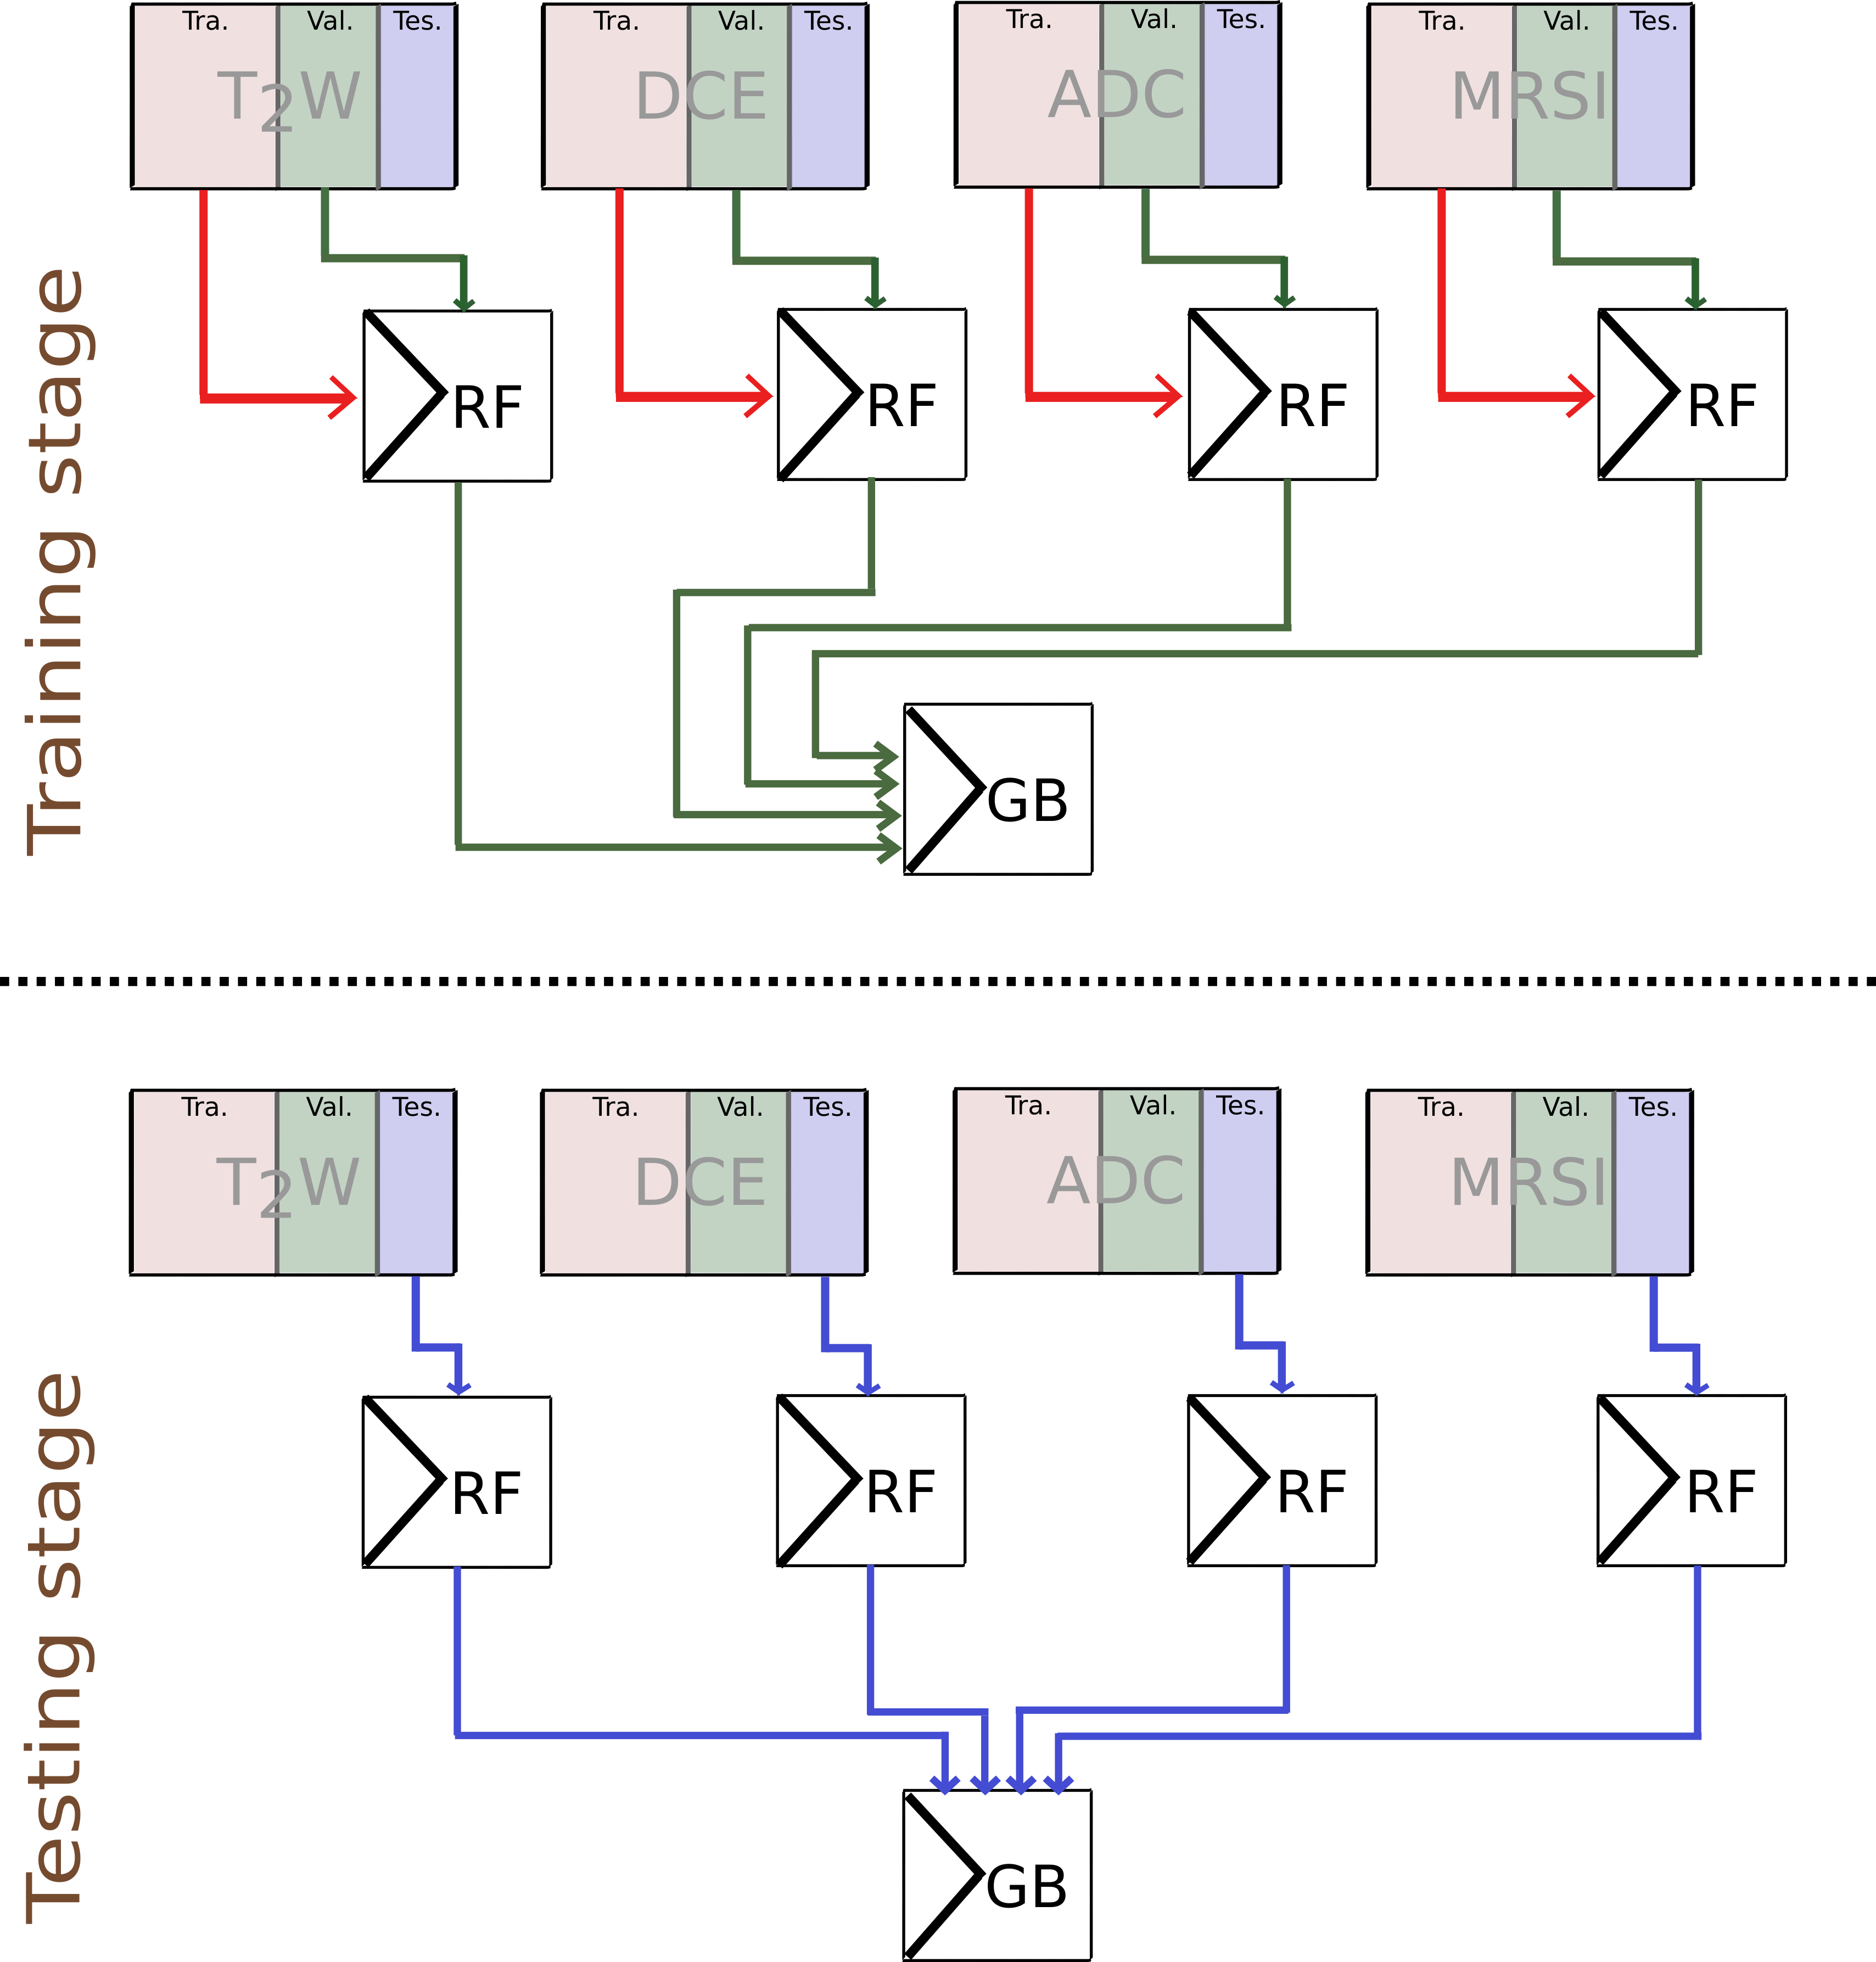
\includegraphics[width=0.5\linewidth]{6_pipeline/figures/stacking_gb.png}
  \caption[The principle of stacking.]{The principle of stacking. First, training samples (red) are used to train each individual \ac{rf}. Subsequently, a validation set (green) is provided to each \ac{rf} which output a set of probability used for the classification of the meta-classifier. Finally, a test set is used to asses the classification performance to whole stack.}
  \label{fig:stacking}
\end{figure}

Additionally, we will use stacking is a way to create a meta classifier using different base learners~\cite{wolpert1992stacked}.
This method uses the prediction of different base learners as input for a meta leaner and combines them into a final decision.
Each base learner is trained on the training set and its prediction on the validation set is fed to the meta learner.
The test sample, in a similar way is first classified by the base learners and their prediction is passed through the meta learner in order to achieve the final decision.
 
